\section{Sensitivity Audits and Methodological Robustness}
\label{sec:sensitivity}

To ensure that spatial prioritization decisions and municipal risk classifications are not sensitive artifacts of arbitrary modeling assumptions, we conduct an exhaustive sensitivity and robustness audit across weighting philosophies, non-linear coupling parameters, and stochastic weight perturbations across all 334,332 observations.

\subsection{Weighting Scheme Invariance}
A frequent criticism of composite indices is that relative city or neighborhood rankings can flip depending on whether equal, entropy, or principal component weights are assigned. We compare our pre-registered primary formulation ($\text{SSI}_{\text{equal}}$) against linear composites generated under the Entropy Weight Method ($\text{SSI}_{\text{ewm}}$), CRITIC ($\text{SSI}_{\text{critic}}$), and PCA ($\text{SSI}_{\text{pca}}$) (Table~\ref{tab:weights_comparison}).

Evaluating pairwise spatial rank correlations across all 334,332 hexagonal cells yields:
\begin{equation}
    \rho(\text{Equal}, \text{EWM}) = 0.9691, \quad \rho(\text{Equal}, \text{CRITIC}) = 0.9857, \quad \rho(\text{Equal}, \text{PCA}) = 0.8919
\end{equation}
Minimum Kendall $\tau$ rank concordance exceeds $0.80$ across all comparisons. While alternative schemes slightly shift the absolute magnitude of individual scores (e.g., EWM places higher weight on high-dispersion winter smog, while PCA elevates summer heat-water covariance), \textbf{spatial cell rankings are over $89\%\text{--}98\%$ invariant to the weighting philosophy chosen}. This demonstrates that our equal-weight baseline provides an objective, transparent foundation without distorting municipal vulnerability prioritizations.

\subsection{Coupling Intensity \texorpdfstring{($\gamma$)}{(gamma)} and Quantile Threshold \texorpdfstring{($q$)}{(q)} Sweeps}
The non-linear compound interaction is governed by two hyperparameters: the coupling intensity $\gamma$ (pre-registered at $0.30$) and the joint-tail quantile threshold $q$ (pre-registered at $0.90$). We perform a comprehensive 2D grid sweep across $\gamma \in [0.1, 0.2, 0.3, 0.4, 0.5]$ and $q \in \{0.75, 0.90, 0.95\}$ across all seven metropolitan panels (Figure~\ref{fig:compound_sensitivity}).

\begin{figure*}[t]
    \centering
    \IfFileExists{figures/Figure5_compound_sensitivity.png}{%
        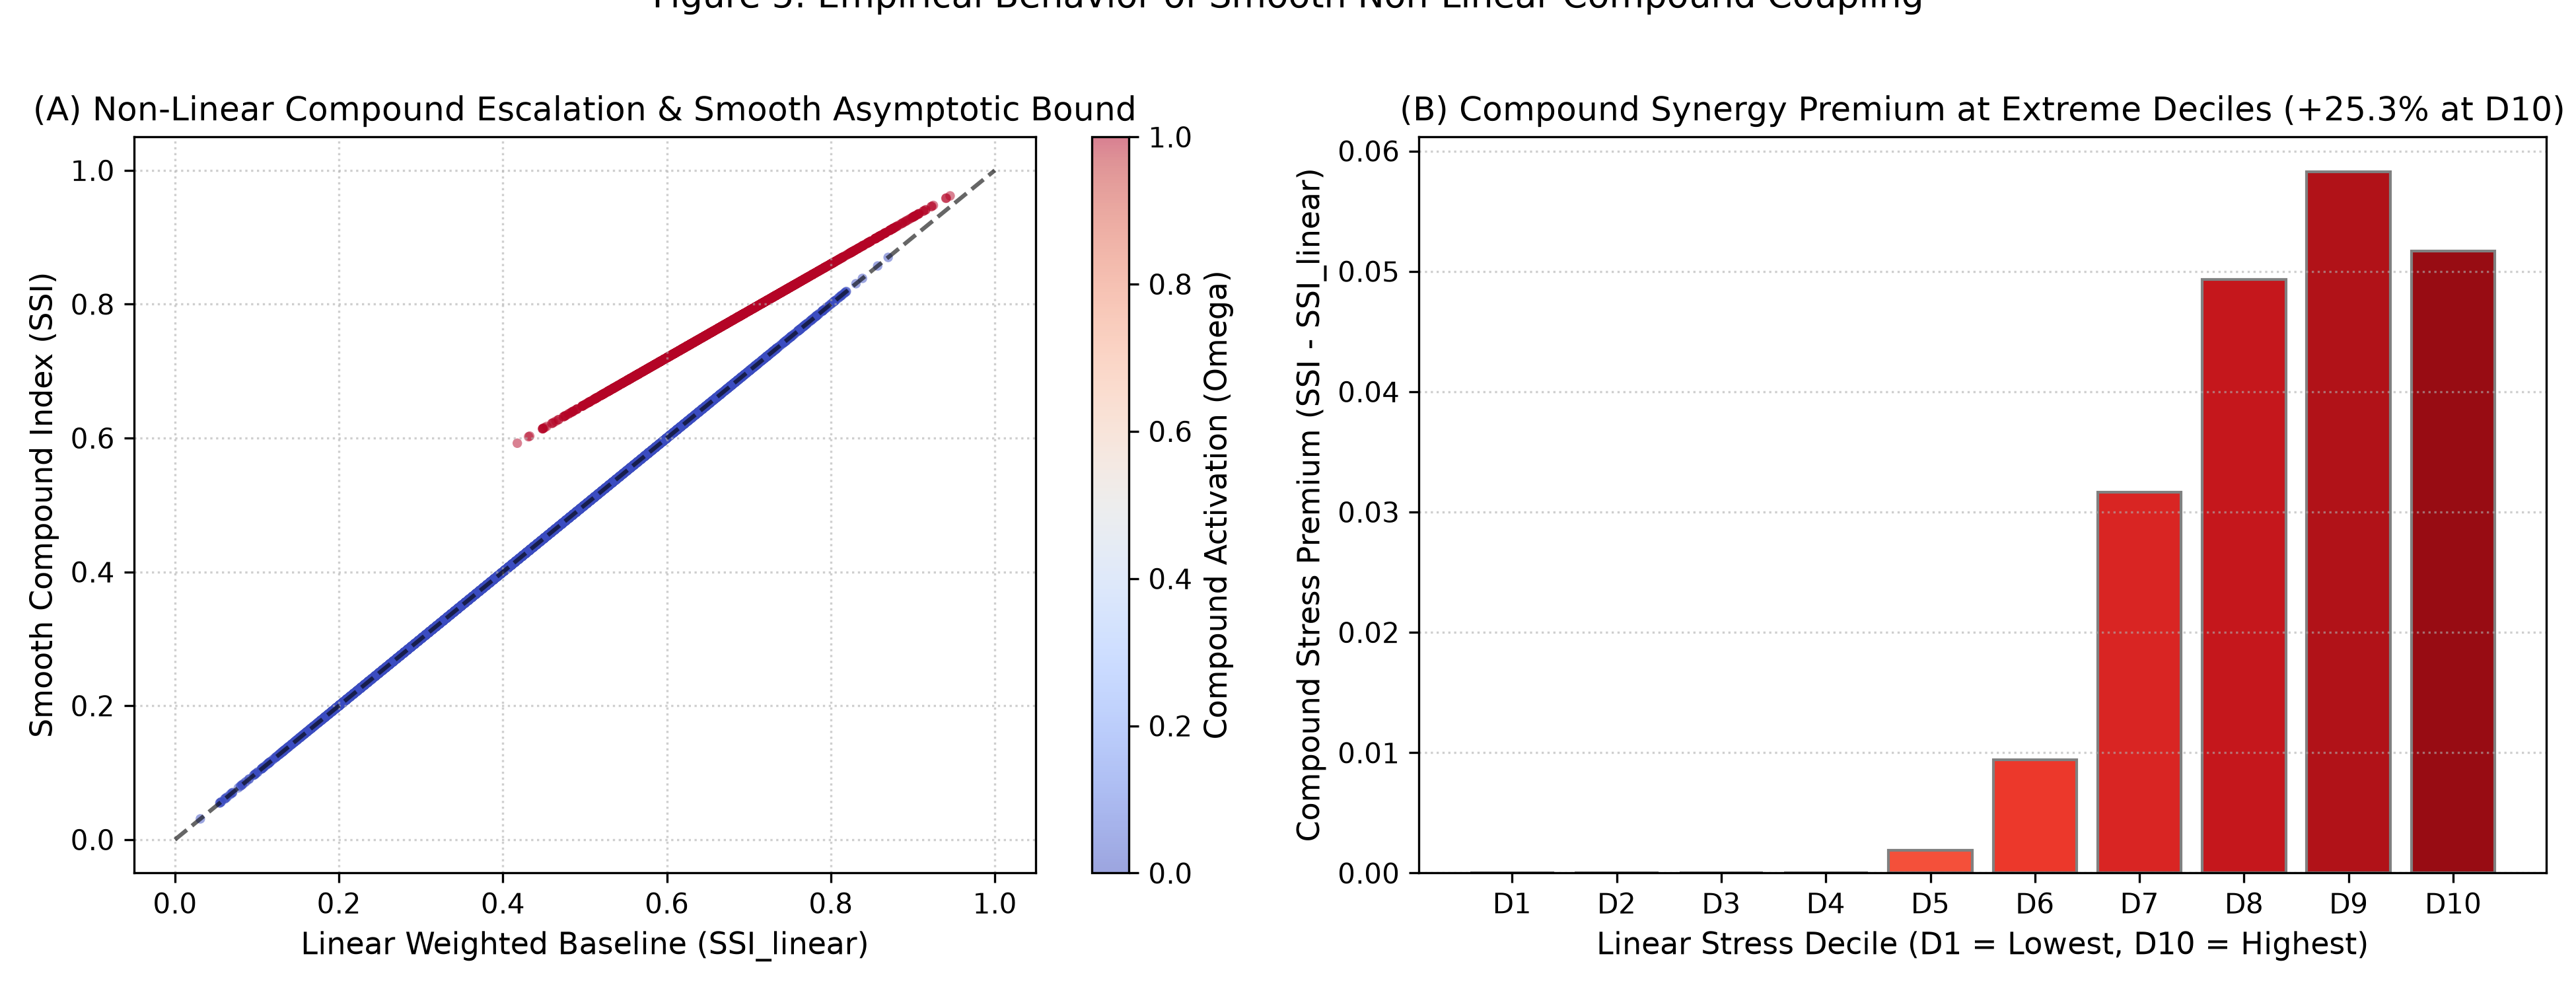
\includegraphics[width=\textwidth]{figures/Figure5_compound_sensitivity.png}%
    }{%
        \vspace{1em}
        \fbox{\parbox{0.95\textwidth}{\centering\small\textbf{[Figure 5: Compound Interaction Coupling and Decile Amplification]}\\
        \textit{Generated via \texttt{colab\_analysis.py} from \texttt{final\_7\_cities.parquet} ($N = 334,332$). (A) Non-linear joint-tail escalation vs. linear identity; (B) Decile compound synergy premium showing +25.3\% amplification at D10.}}}%
        \vspace{1em}
    }
    \caption{Empirical verification of smooth asymptotic compound hazard coupling ($N = 334,332$). (A) Scatter plot of linear base vs. compound SSI shaded by joint-tail activation ($\Omega_{\text{compound}}$), confirming smooth upper boundary adherence ($0.00\%$ records clamped at 1.0); (B) Decile stress escalation demonstrating marked compound amplification ($+25.3\%$) concentrated in extreme tail regimes (Decile~10).}
    \label{fig:compound_sensitivity}
\end{figure*}

The results confirm extreme stability:
\begin{itemize}
    \item \textbf{Rank Preservation:} Across all grid configurations, the spatial rank correlation against the primary baseline never drops below \textbf{$\rho = 0.9954$} (minimum $\tau = 0.9734$). Altering $\gamma$ from $0.1$ to $0.5$ shifts absolute index levels monotonically but leaves spatial priority rankings virtually unchanged ($\rho > 0.998$).
    \item \textbf{Activation Rates:} Setting $q = 0.75$ triggers compound interaction across $20.66\%$ of pan-India observations, while the more restrictive tail cutoff $q = 0.90$ cleanly isolates acute multi-hazard crises (e.g., $30.91\%$ in Delhi, $40.44\%$ in Bikaner, and $0.68\%$ in Coimbatore).
\end{itemize}

\subsection{Monte Carlo Random Weight Perturbation}
To evaluate sensitivity to random parametric noise, we execute a 200-run Monte Carlo uncertainty analysis where indicator weights are randomly drawn from a Dirichlet distribution centered on the primary equal weights with a $\pm 25\%$ uniform perturbation window. The mean pairwise Spearman correlation across all perturbed indices is \textbf{$\rho = 0.9975 \pm 0.0018$}, verifying that the index is immune to minor weighting adjustments.
